\documentclass[11pt,a4paper]{article}

\usepackage[T1]{fontenc}
\usepackage{lmodern}
\usepackage[utf8]{inputenc}
\usepackage[margin=1in]{geometry}
\usepackage{booktabs}
\usepackage{graphicx}
\usepackage{amsmath}
\usepackage{siunitx}
\usepackage{microtype}
\usepackage[hidelinks]{hyperref}
\usepackage{caption}
% \FloatBarrier keeps a table ahead of the text that discusses it
\usepackage{placeins}

\sisetup{group-separator={,}}
\captionsetup{font=small,labelfont=bf}
\setlength{\parskip}{0.4em}
\setlength{\parindent}{0pt}
% long unbreakable \texttt{} filenames would otherwise overflow the margin
\setlength{\emergencystretch}{3em}

\begin{document}

\begin{titlepage}
\centering
\vspace*{0.22\textheight}
{\LARGE\bfseries Who Reports Withdrawal Dates in the Western\\[0.3em]
Interconnection Queue, and Does It Matter?\par}
\vspace{3em}
{\Large Noah Parsons\par}
\vspace{0.8em}
{\large Independent Researcher\par}
\vspace{0.8em}
\href{mailto:parsons.m.noah@gmail.com}{\texttt{parsons.m.noah@gmail.com}}\par
\vspace{0.3em}
ORCID: \href{https://orcid.org/0009-0000-7224-6040}{0009-0000-7224-6040}\par
\vfill
{\large Working paper, September 2026\par}
\vspace{0.5em}
DOI: \href{https://doi.org/10.5281/zenodo.22547678}{10.5281/zenodo.22547678}\par
\vspace{2em}
\end{titlepage}

\begin{abstract}
\noindent
Berkeley Lab's \emph{Queued Up} publishes a median duration from interconnection
request to withdrawal for the non-ISO West. That figure is computed from the
\SI{12.1}{\percent} of western withdrawals carrying a recorded withdrawal date:
636 of \num{5277}. This paper asks whether those records represent the region
they describe. They do not---technology mix, queue cohort and interconnection
service type all differ from the regional population at $p < 10^{-10}$, while
project capacity does not. But standardising the subset to the region's actual
composition moves the median by less than three months, with an interval
including zero and a sign that reverses under a truncation-matched observation
window. A validation exercise inside the well-covered ISO regions explains why:
imposing the West's compositional distortion on a population whose durations are
fully observed shifts the median by about eight days. Technology, cohort and
capacity together explain \SI{4.6}{\percent} of the variance in withdrawal
duration, leaving coverage rather than composition as the binding caveat. A
companion logistic regression over the \num{7991} western requests with complete
predictors, requiring no dates, finds solar the most withdrawal-prone technology, larger projects likelier
to be withdrawn, and roughly a quarter of the latent variation in withdrawal risk
sitting between providers rather than between projects.
\end{abstract}

\section*{Summary}

Berkeley Lab's \emph{Queued Up} series publishes, among much else, a median
duration from interconnection request to withdrawal for each region of the
United States. For the non-ISO West that figure is computed from the withdrawals
that carry a recorded withdrawal date. In the 2026 Edition data file, that is 636
of \num{5277} western withdrawals---\textbf{\SI{12.1}{\percent}}. The remaining
\SI{87.9}{\percent} are known to have been withdrawn but not when.

This paper asks whether those 636 records are representative of the region whose
duration they are used to describe, and if not, how far the published median is
displaced as a result. The answer has three parts.

\textbf{First, the reporting is extraordinarily concentrated.} Of the 31 western
transmission providers with at least one withdrawal in the file, six record any
withdrawal date at all and five record one for more than a quarter of their
withdrawals. PacifiCorp---which alone accounts for \num{2160} of the region's
\num{8097} requests and \num{1627} of its withdrawals, more than twice the
next-largest provider on either count---records a date for \SI{6.0}{\percent} of
them. The median western withdrawal duration is, in practice, a statistic about
Colorado, New Mexico, eastern Washington, Los Angeles and El Paso.

\textbf{Second, that subset is compositionally unlike the region.} Technology
mix, queue cohort and interconnection service type all differ from the regional
population at $p < 10^{-10}$ after correction for multiple comparisons, on both
of the two defensible definitions of ``the reporting subset.'' Project capacity
does not differ. The dated records over-represent stand-alone solar
(\SI{44.8}{\percent} against \SI{31.5}{\percent}) and wind (\SI{30.7}{\percent}
against \SI{23.1}{\percent}) and under-represent solar-plus-storage
(\SI{10.7}{\percent} against \SI{18.8}{\percent}) and stand-alone storage
(\SI{3.6}{\percent} against \SI{9.0}{\percent}).

\textbf{Third---and this is the part that resists the obvious conclusion---those
compositional differences barely move the median.} Standardising the reporting
subset to the region's actual technology-by-cohort composition shifts the median
by $-0.06$ years, with a \SI{95}{\percent} bootstrap interval of $[-0.23,
+0.00]$. Under a truncation-matched window the shift is $+0.19$ years. The sign
flips. A validation exercise inside the ISO regions, where date coverage is
near-complete and the answer is therefore known, shows why: deliberately imposing
the West's skewed composition on those regions biases their median by $0.021$
years---about eight days. Technology, cohort and capacity together explain
\SI{4.6}{\percent} of the variance in withdrawal duration where it can be
measured well. Composition is simply not a strong enough determinant of duration
for a composition gap of this size to matter much.

The correct caveat on the published western median is therefore not ``it is
biased by an unrepresentative technology mix.'' It is ``it is computed from one
eighth of the region's withdrawals, drawn from five of thirty-one providers, and
the mechanism by which that might bias it is unmeasured.'' Composition is the
part we can check, and it is small. What we cannot check is whether providers
that record dates withdraw on a different \emph{schedule} from providers that do
not---and nothing in this data file can settle that.

\section{The question}

Interconnection queues have become the binding constraint on adding generation to
the North American grid, and \emph{Queued Up} is the reference description of
them. Its regional summaries are widely cited in regulatory filings, trade press
and academic work. One of those summaries is the typical time a request spends in
the queue before being withdrawn---a natural measure of how much developer effort
the process absorbs before yielding nothing.

Computing that statistic requires two dates: when the request entered the queue,
and when it was withdrawn. The first is recorded almost universally. The second
is not. Transmission providers publish their queues in whatever format they
choose, and many simply drop a withdrawn request from the published list without
recording the date on which it left. The compilers of \emph{Queued Up} can only
report what providers publish.

Where coverage is near-complete this is a non-issue. In the four regions with the
best coverage---ISO-NE, CAISO, PJM and MISO---\SIrange{94}{99}{\percent} of
withdrawals carry a date, so the observed durations are effectively a census. In
the non-ISO West they are \SI{12.1}{\percent} of withdrawals, and the question of
who those \SI{12.1}{\percent} are becomes unavoidable.

Two things could go wrong. The reporting subset could differ from the region in
project characteristics that themselves influence how long a request survives---a
subset heavy in wind, say, when wind takes longer to withdraw than solar. Call
this \textbf{compositional bias}; it is measurable, because both the composition
of the subset and the composition of the region are observed. Or the providers
that record dates could simply process requests differently from those that do
not, in ways not captured by any recorded project attribute. Call this
\textbf{provider process bias}; it is not measurable from this file, because the
durations of the non-reporting providers are exactly what is missing.

This paper measures the first and bounds what can be said about the second.

\section{Data}

The analysis uses a single source: the \emph{Queued Up} 2026 Edition data file
(\texttt{LBNL\_Ix\_Queue\_Data\_File\_thru2025.xlsx}), covering interconnection
requests through the end of 2025, published by Lawrence Berkeley National
Laboratory and GridTracker under CC BY 4.0. Sheet \texttt{03. Complete Queue
Data} holds project-level records: \num{38201} rows across nine regions.

The \texttt{region} field distinguishes the seven ISO/RTO territories, the
Southeast, and ``West''---the non-ISO Western Interconnection within the United
States, i.e.\ the US portion of WECC excluding CAISO; the file contains no
Canadian or Mexican records. That western region is the study population:
\textbf{\num{8097} requests}, of which \num{5277} (\SI{65.2}{\percent}) are
recorded as withdrawn, \num{1603} active, 963 operational, 244 suspended and 10
unknown.

Four fields carry the analysis. \texttt{q\_date} and \texttt{wd\_date} give the
request and withdrawal dates; their difference, in years, is the duration.
\texttt{type\_clean} gives a cleaned technology label, which I collapse to six
groups (Solar, Wind, Solar+Battery, Battery, Gas, Other). \texttt{q\_year} gives
the queue entry year, binned into four cohorts ($\leq$2014, 2015--18, 2019--21,
2022+). \texttt{mw\_1} gives nameplate capacity, and \texttt{entity} the
transmission provider.

A record is \textbf{dated} if it carries both a queue date and a withdrawal date
and the resulting duration is non-negative. Six records across the whole file
have withdrawal dates preceding their queue dates and are excluded on that
ground. By this definition 636 of the West's \num{5277} withdrawals are dated.
Ten western withdrawals carry neither a queue date nor a queue year. None of them
is dated, but none can be assigned a cohort either, so the cohort-stratified
analyses in Sections~4 and~\ref{sec:standardise} take as their regional
population the remaining \num{5267} withdrawals. All 636 dated records are
retained throughout.

Two definitions of ``the reporting subset'' are carried in parallel throughout,
because they are not the same set and the choice turns out to matter more than
any of the corrections applied to them:

\begin{itemize}
\item \textbf{dated records}---the 636 withdrawn requests carrying a usable
duration. This is what the published median literally rests on, irrespective of
who filed them.
\item \textbf{reporting entities}---the 539 dated withdrawals filed with the five
providers that record a date for at least a quarter of their withdrawals. This is
the institutional unit: the set of providers whose reporting practice makes the
statistic possible.
\end{itemize}

The gap between them is exactly 97 dated records, every one of them PacifiCorp's.

\begin{table}[htbp]
\centering
\caption{Withdrawal-date coverage by region.}
\begin{tabular}{lrrr}
\toprule
Region & Withdrawals & Dated & Coverage \\
\midrule
ISO-NE      & \num{982}  & \num{970}  & \SI{98.8}{\percent} \\
CAISO       & \num{2200} & \num{2160} & \SI{98.2}{\percent} \\
PJM         & \num{5226} & \num{5091} & \SI{97.4}{\percent} \\
MISO        & \num{3263} & \num{3060} & \SI{93.8}{\percent} \\
SPP         & \num{1846} & \num{1340} & \SI{72.6}{\percent} \\
NYISO       & \num{1531} & \num{745}  & \SI{48.7}{\percent} \\
ERCOT       & \num{1158} & \num{520}  & \SI{44.9}{\percent} \\
Southeast   & \num{2738} & \num{845}  & \SI{30.9}{\percent} \\
\textbf{West} & \textbf{\num{5277}} & \textbf{636} & \textbf{\SI{12.1}{\percent}} \\
\bottomrule
\end{tabular}
\end{table}

The West is not merely the worst-covered region; it is worse by a factor of two
and a half than the next-worst. This ordering also defines the calibration set
used in Section~\ref{sec:standardise}: the four regions above
\SI{90}{\percent} coverage.

\section{The roster}

The concentration of reporting is the single most striking feature of the western
data, and it is worth setting out in full before any modelling.

Thirty-six entities appear in the western region. Five have no withdrawals at
all. Of the remaining 31, \textbf{six record at least one withdrawal date, and
five record one for at least a quarter of their withdrawals.}

\begin{table}[htbp]
\centering
\caption{Western transmission providers with 25 or more requests, through 2025.
\emph{Dated} counts withdrawals carrying a usable duration; \emph{Rate} is that
as a share of the provider's withdrawals. Reporting providers in bold. The
remaining nine providers have fewer than 25 requests each and none records a
date.}
\begin{tabular}{lrrrr}
\toprule
Provider & Requests & Withdrawn & Dated & Rate \\
\midrule
PacifiCorp        & \num{2160} & \num{1627} & 97  & \SI{6.0}{\percent} \\
BPA               & \num{998}  & \num{611}  & 0   & \SI{0}{\percent} \\
Idaho Power       & \num{824}  & \num{515}  & 0   & \SI{0}{\percent} \\
APS               & \num{619}  & \num{426}  & 0   & \SI{0}{\percent} \\
NV Energy         & \num{505}  & \num{263}  & 0   & \SI{0}{\percent} \\
NorthWestern      & \num{448}  & \num{328}  & 0   & \SI{0}{\percent} \\
\textbf{PSCo}     & \num{408}  & \num{295}  & \num{285} & \textbf{\SI{96.6}{\percent}} \\
\textbf{PNM}      & \num{356}  & \num{224}  & \num{133} & \textbf{\SI{59.4}{\percent}} \\
WAPA-IS           & \num{273}  & \num{194}  & 0   & \SI{0}{\percent} \\
\textbf{Avista}   & \num{173}  & \num{117}  & 71  & \textbf{\SI{60.7}{\percent}} \\
SRP               & \num{155}  & \num{105}  & 0   & \SI{0}{\percent} \\
PSE               & \num{142}  & \num{86}   & 0   & \SI{0}{\percent} \\
TEP               & \num{120}  & \num{84}   & 0   & \SI{0}{\percent} \\
PGE               & \num{114}  & \num{51}   & 0   & \SI{0}{\percent} \\
\textbf{LADWP}    & \num{113}  & \num{55}   & 36  & \textbf{\SI{65.5}{\percent}} \\
WAPA-RM           & \num{110}  & \num{88}   & 0   & \SI{0}{\percent} \\
TSGT              & \num{104}  & \num{14}   & 0   & \SI{0}{\percent} \\
\textbf{EPE}      & \num{66}   & \num{30}   & 14  & \textbf{\SI{46.7}{\percent}} \\
PRPA              & \num{62}   & \num{35}   & 0   & \SI{0}{\percent} \\
BHCT              & \num{51}   & \num{32}   & 0   & \SI{0}{\percent} \\
SRP-ANPP          & \num{45}   & \num{18}   & 0   & \SI{0}{\percent} \\
CLPT              & \num{40}   & \num{13}   & 0   & \SI{0}{\percent} \\
WAPA-DSW          & \num{34}   & 0          & 0   & --- \\
IID               & \num{33}   & 0          & 0   & --- \\
SMUD              & \num{33}   & \num{18}   & 0   & \SI{0}{\percent} \\
SRP-PV/PC         & \num{33}   & \num{22}   & 0   & \SI{0}{\percent} \\
BHP               & \num{26}   & \num{7}    & 0   & \SI{0}{\percent} \\
\bottomrule
\end{tabular}
\end{table}
\FloatBarrier

The distribution is close to binary. Providers either record dates for roughly
half their withdrawals or better, or they record none whatsoever. PacifiCorp is
the sole exception, and its \SI{6.0}{\percent} is the reason the count of
reporting providers reads six or five depending on where the line is drawn---a
distinction with real consequences, since PacifiCorp is by a wide margin the
largest queue in the region.

That PacifiCorp is both the largest western queue and a near-total non-reporter
is the central fact of this paper. Its \num{1627} withdrawals are
\SI{31}{\percent} of the region's total, and 2.7 times those of the next-largest
provider. Yet its 97 dated records are only \SI{15}{\percent} of the 636 on which
the published median rests, and they are a \SI{6}{\percent} sample of its own
withdrawals. Whatever the typical PacifiCorp withdrawal duration is, the
published median sees it only through that sample.

Note also the geographic consequence. The five reporting providers serve Colorado
(PSCo), New Mexico and west Texas (PNM, EPE), eastern Washington and northern
Idaho (Avista), and the City of Los Angeles (LADWP). The published western median
describes those service territories. It is nearly silent on Oregon, Montana,
Wyoming, Nevada, Arizona and the Bonneville footprint. I do not report a formal
test of geographic difference, because provider and state are so nearly collinear
in this region that such a test would only restate Table~2.

\begin{figure}[htbp]
\centering
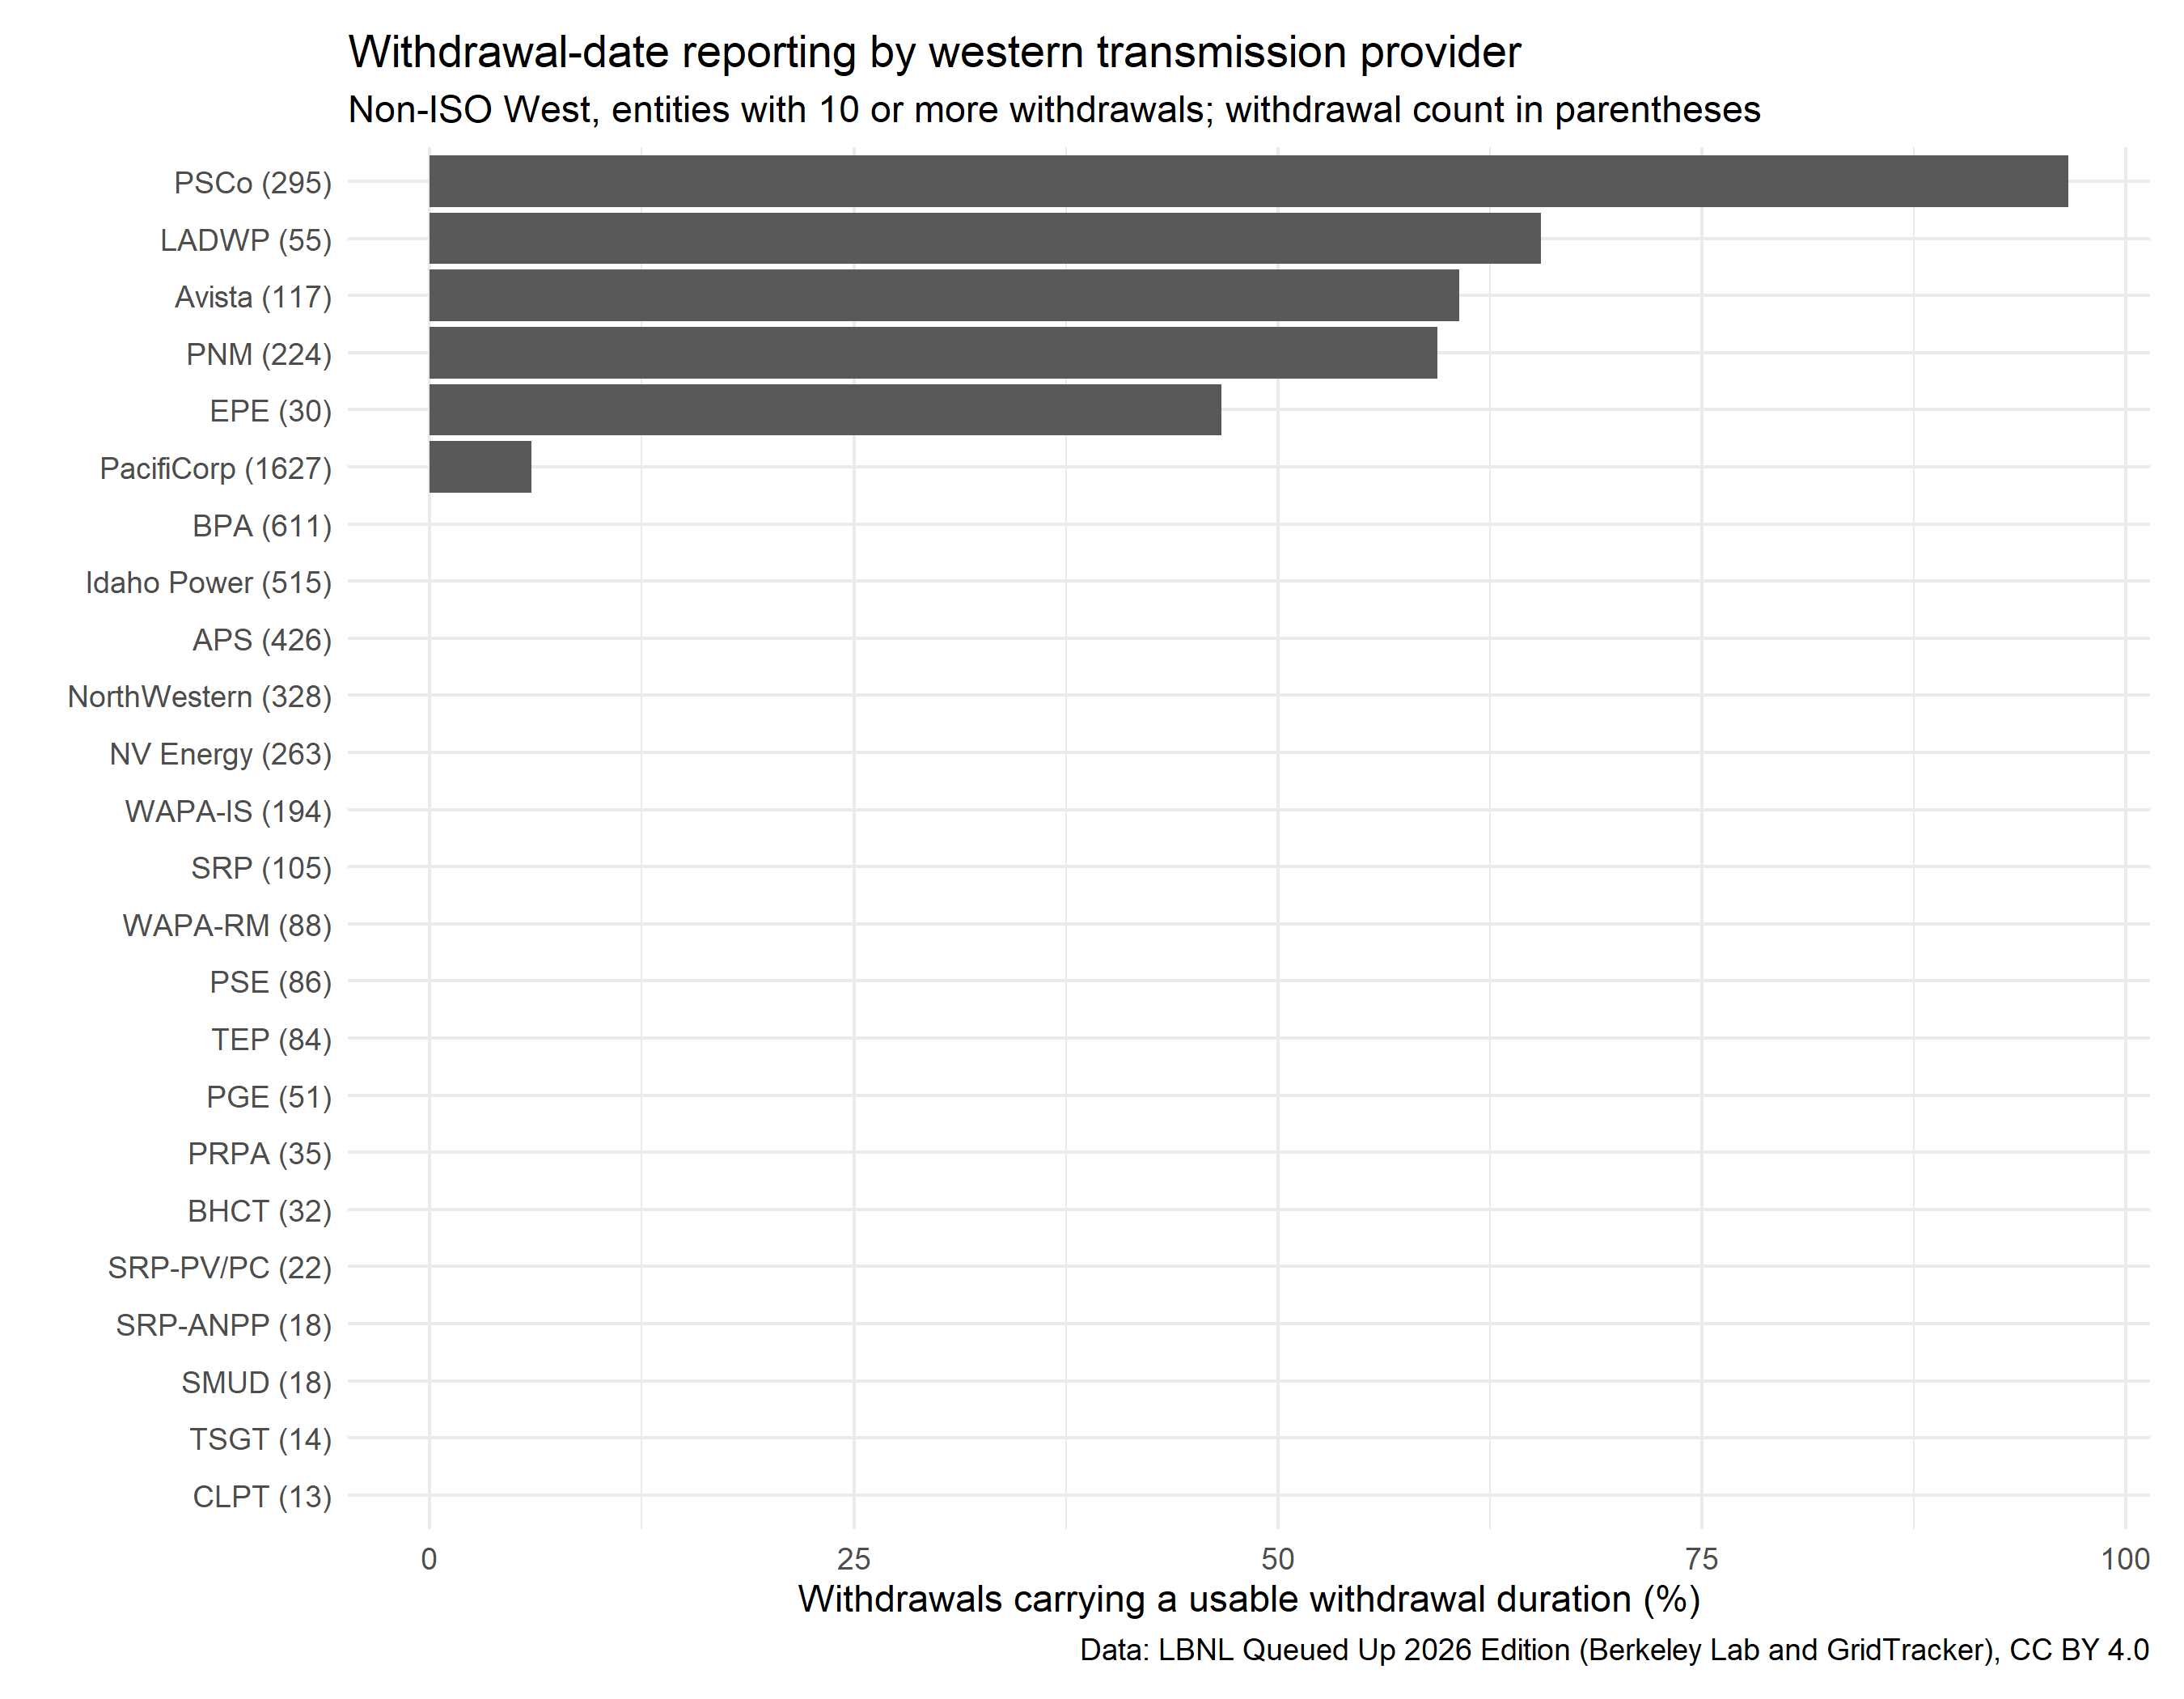
\includegraphics[width=\textwidth]{figures/01-reporting-by-entity.png}
\caption{Withdrawal-date reporting rate by western transmission provider,
for providers with ten or more withdrawals.}
\end{figure}

\section{Is the reporting subset different?}

\subsection{Method}

I test five pre-specified comparisons between the reporting subset and the rest
of the region. Four are project attributes that the ISO calibration in
Section~\ref{sec:standardise} shows to influence duration; the fifth is a
provider-level property.

\begin{enumerate}
\item \textbf{Technology mix}---six groups, Pearson $\chi^2$.
\item \textbf{Queue cohort mix}---four bins, Pearson $\chi^2$.
\item \textbf{Capacity}---\texttt{mw\_1}, Wilcoxon rank-sum.
\item \textbf{Interconnection service type}---ERIS / NRIS / NRIS-ERIS / Other,
$\chi^2$.
\item \textbf{Withdrawal rate}---the share of all requests ending in withdrawal,
$\chi^2$, computed over all \num{8097} requests rather than the withdrawals
alone.
\end{enumerate}

Each family of five is Holm-corrected within basis. Both bases receive the full
family, giving ten tests in all. For test 5 each basis takes its natural
provider-level analogue: for the dated basis, providers recording any date (six,
including PacifiCorp); for the entity basis, providers clearing the
\SI{25}{\percent} threshold (five).

Each test compares the reporting subset with the \emph{remainder} of the region.
The composition shares quoted in Section~4.2 and shown in Figure~2 are instead
set against the \emph{whole} regional population, subset included, since that is
the population the published median is taken to describe.

\subsection{Results}

\begin{table}[htbp]
\centering
\caption{The family of five comparisons, Holm-adjusted within basis.}
\begin{tabular}{llrrl}
\toprule
Basis & Comparison & Statistic & $p$ (Holm) & Verdict \\
\midrule
dated records & technology mix   & $\chi^2 = 129.04$ & $1.9\times10^{-25}$ & \textbf{difference} \\
dated records & queue cohort mix & $\chi^2 = 70.70$  & $9.1\times10^{-15}$ & \textbf{difference} \\
dated records & capacity (MW)    & $W = \num{1466743}$ & $0.80$ & null \\
dated records & service type     & $\chi^2 = 54.19$  & $2.0\times10^{-11}$ & \textbf{difference} \\
dated records & withdrawal rate  & $\chi^2 = 101.95$ & $2.3\times10^{-23}$ & \textbf{difference} \\
\midrule
reporting entities & technology mix   & $\chi^2 = 120.19$ & $1.1\times10^{-23}$ & \textbf{difference} \\
reporting entities & queue cohort mix & $\chi^2 = 142.76$ & $4.8\times10^{-30}$ & \textbf{difference} \\
reporting entities & capacity (MW)    & $W = \num{1562008}$ & $0.068$ & null \\
reporting entities & service type     & $\chi^2 = 58.54$  & $3.6\times10^{-12}$ & \textbf{difference} \\
reporting entities & withdrawal rate  & $\chi^2 = 0.16$   & $0.69$ & null \\
\bottomrule
\end{tabular}
\end{table}

Three comparisons return a difference on both bases: \textbf{technology mix,
queue cohort mix and interconnection service type}. One returns a null on both:
\textbf{capacity}. One splits: \textbf{withdrawal rate}.

The split is instructive rather than awkward. Providers recording any date
withdraw \SI{71.7}{\percent} of their requests against \SI{60.8}{\percent} for
the rest---but that gap is entirely PacifiCorp, whose own withdrawal rate is
\SI{75.3}{\percent} and whose \num{2160} requests dominate the group. Restrict to
the five genuine reporters and the rates are \SI{64.6}{\percent} against
\SI{65.3}{\percent}, a difference of seven tenths of a percentage point
($p = 0.69$). Providers that actually report dates do not withdraw at an unusual
rate. The apparent effect on the wider definition is one large utility's
idiosyncrasy.

Against the regional population of \num{5267} withdrawals, the 636 dated records
over-represent stand-alone solar (\SI{44.8}{\percent} against
\SI{31.5}{\percent}) and wind (\SI{30.7}{\percent} against \SI{23.1}{\percent}),
and under-represent solar-plus-storage (\SI{10.7}{\percent} against
\SI{18.8}{\percent}), stand-alone storage (\SI{3.6}{\percent} against
\SI{9.0}{\percent}), gas (\SI{3.5}{\percent} against \SI{6.5}{\percent}) and
other technologies (\SI{6.8}{\percent} against \SI{11.2}{\percent}). On cohort
they are close on the oldest bin (\SI{39.3}{\percent} against
\SI{39.6}{\percent}) but over-represent 2019--21 (\SI{22.2}{\percent} against
\SI{14.6}{\percent}) and under-represent 2022 and later (\SI{14.3}{\percent}
against \SI{25.7}{\percent}).

The shape of this is coherent. Storage and hybrid projects entered western queues
in volume from about 2019, and did so disproportionately in the territories of
the large non-reporting providers. The reporting subset is therefore both older
and more conventional in technology than the region it stands for.

\begin{figure}[htbp]
\centering
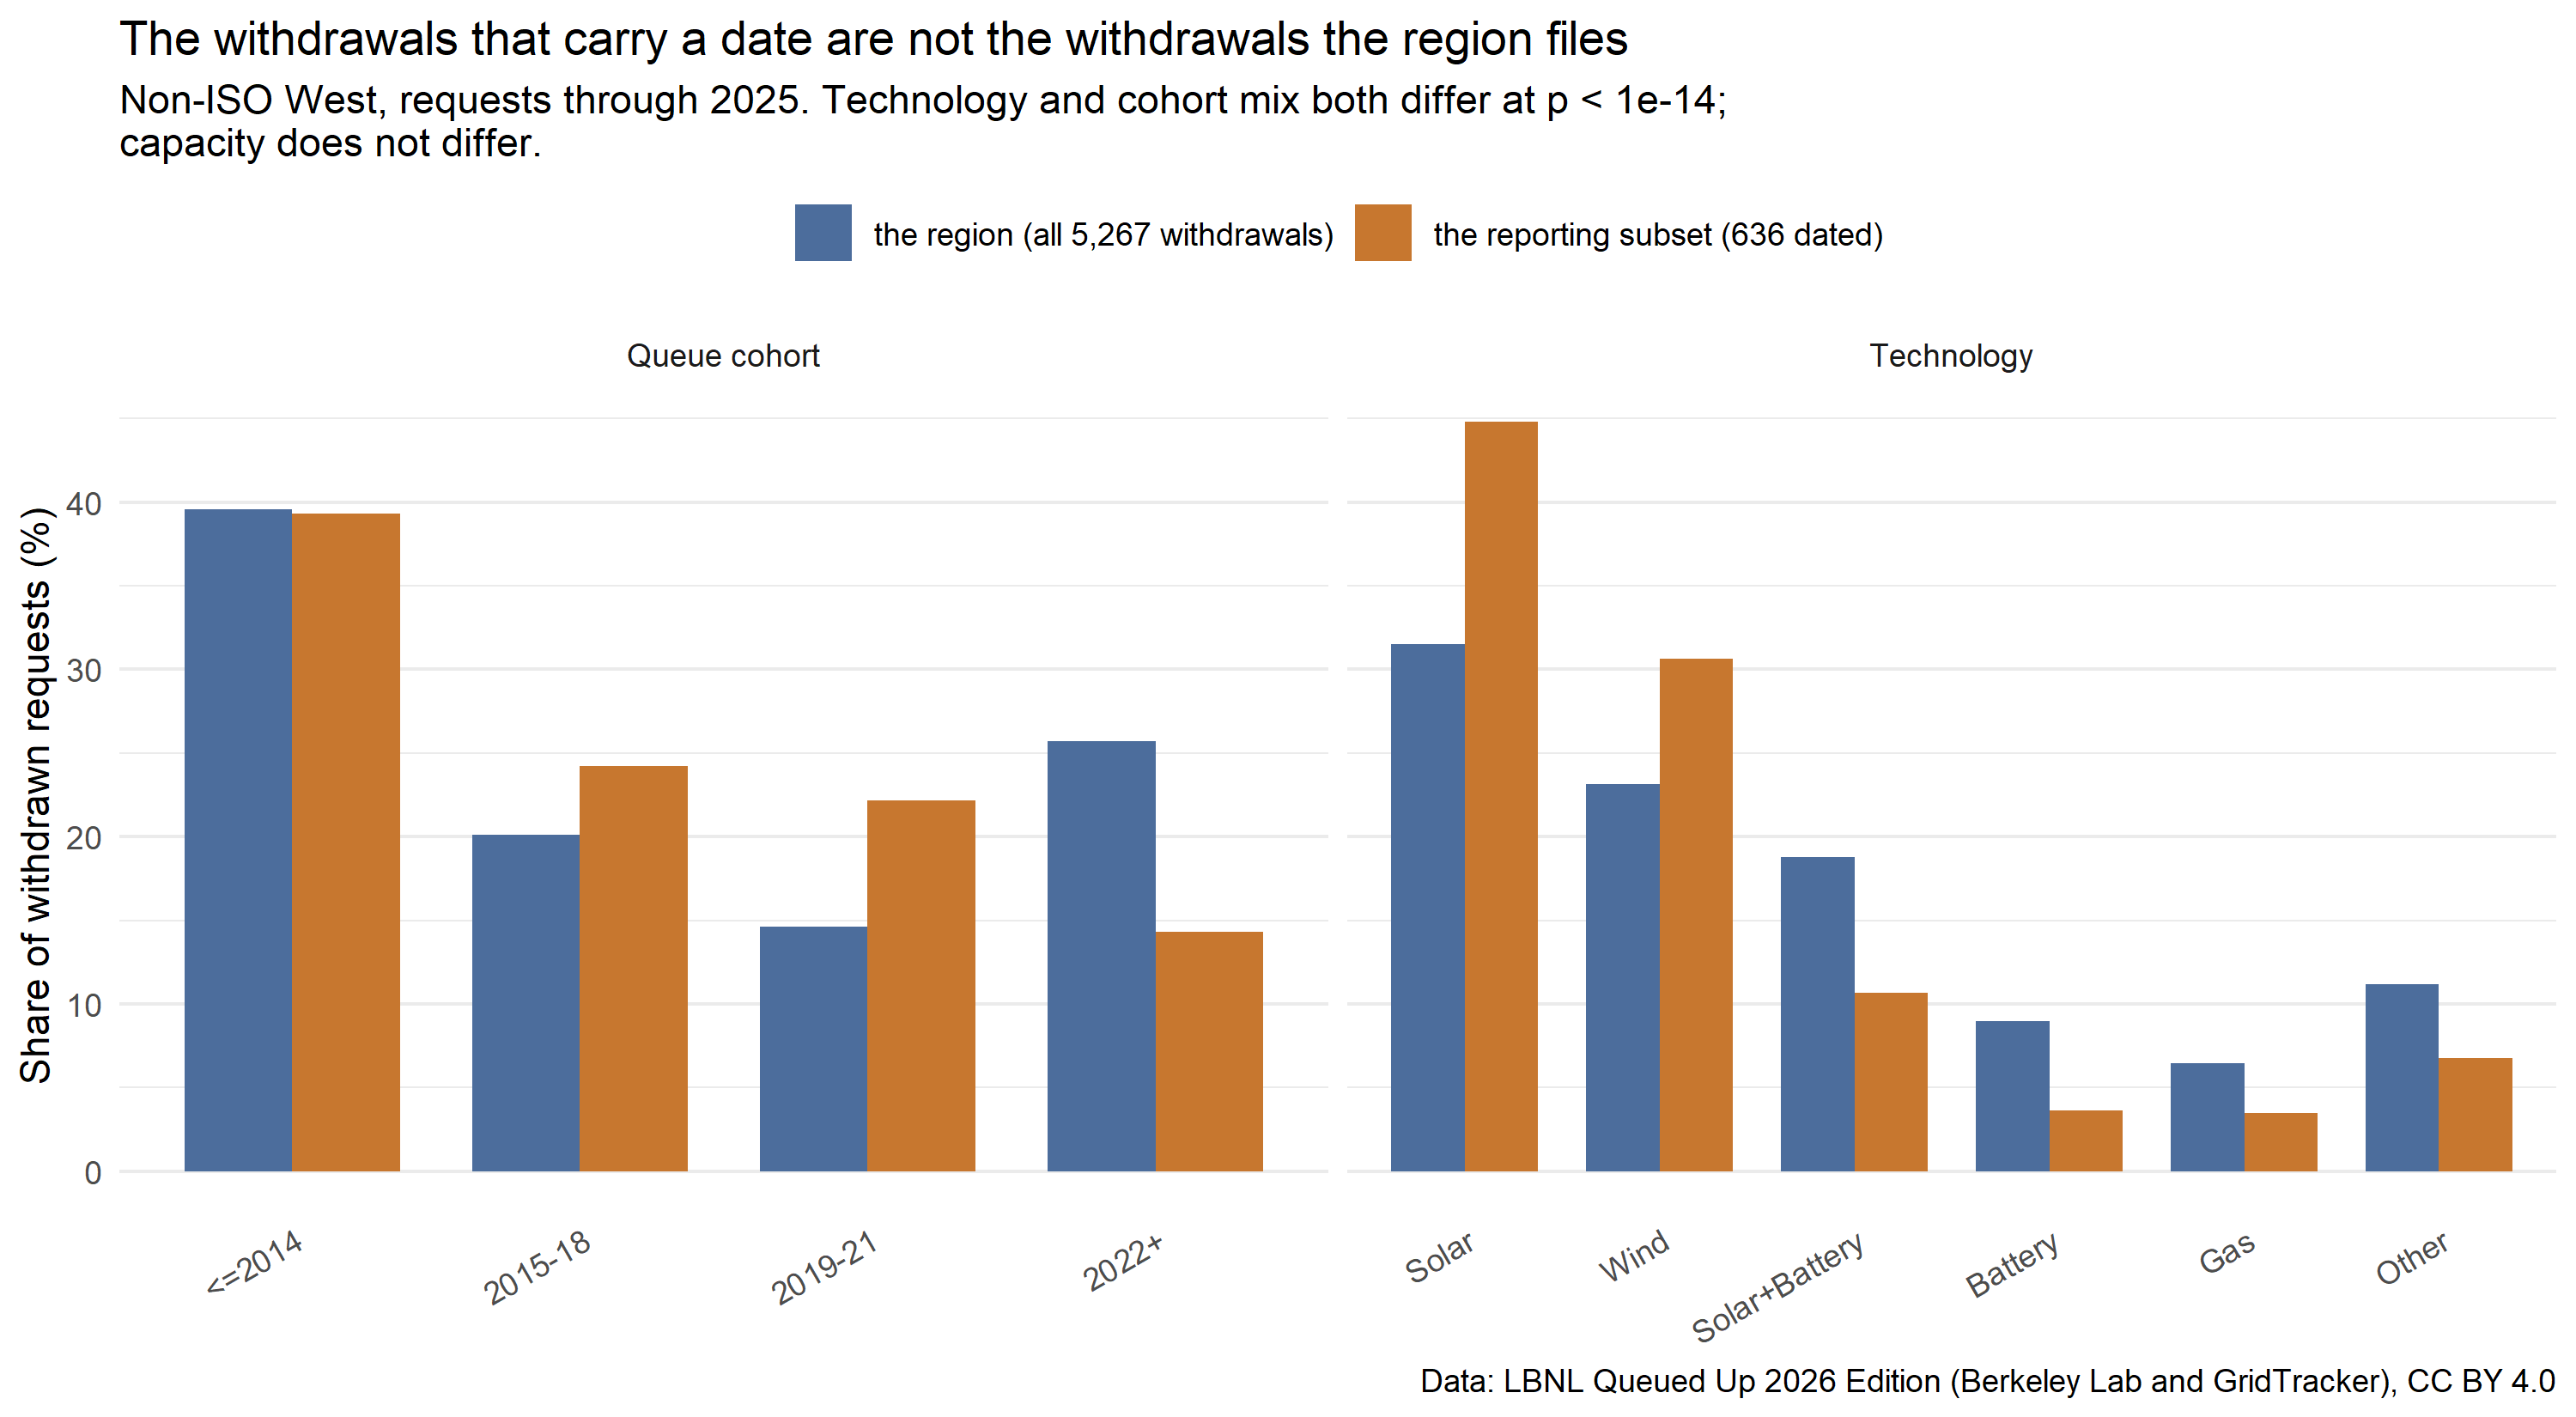
\includegraphics[width=\textwidth]{figures/04-composition-gap.png}
\caption{Technology and queue-cohort composition of the reporting subset against
the region it represents.}
\end{figure}

\section{How far does the composition gap move the median?}
\label{sec:standardise}

Establishing that the reporting subset is unrepresentative does not establish
that the published median is wrong. That requires knowing how strongly the
attributes that differ actually influence duration---and then reweighting.

The estimation proceeds in three stages: calibrate the influence of technology
and cohort on duration where coverage is good; validate the reweighting estimator
in that same place, where the true answer is known; then apply it to the West.

\subsection{Stage A: what moves duration, measured where we can see it}

The four regions above \SI{90}{\percent} coverage---CAISO, ISO-NE, MISO,
PJM---supply \num{11281} dated withdrawals whose durations are effectively a
census rather than a sample. Regressing $\log(\text{duration} + 1/12)$ on
technology, cohort and log capacity there gives the effects in Table~4.

\begin{table}[htbp]
\centering
\caption{ISO calibration ($n = \num{11281}$). Multiplicative effect on duration.}
\begin{tabular}{lrr}
\toprule
Term & Multiplier & $p$ \\
\midrule
Wind (vs Solar)            & 1.447 & $1.5\times10^{-34}$ \\
Solar+Battery              & 1.144 & $7.1\times10^{-5}$ \\
Other                      & 1.076 & $0.043$ \\
Battery                    & 1.031 & $0.27$ \\
Gas                        & 1.005 & $0.88$ \\
cohort 2015--18 (vs $\leq$2014) & 0.849 & $2.4\times10^{-9}$ \\
cohort 2019--21            & 1.420 & $6.1\times10^{-37}$ \\
cohort 2022+               & 1.102 & $0.0022$ \\
log capacity (MW)          & 1.016 & $0.012$ \\
\bottomrule
\end{tabular}
\end{table}
\FloatBarrier

Wind withdrawals take about \SI{45}{\percent} longer than solar; the 2019--21
cohort---the queue surge that has been working through withdrawal since roughly
2024---takes about \SI{42}{\percent} longer than the pre-2015 cohorts. These are
precisely estimated and substantively real.

\textbf{But the model's $R^2$ is 0.046.} Technology, cohort and size together
account for under \SI{5}{\percent} of the variance in how long a request takes to
be withdrawn, in the data where we can measure that variance cleanly. This single
number governs everything that follows: composition can differ a great deal
without the median moving much, because composition is a weak determinant of
duration.

\subsection{Stage B: does the correction work where the answer is known?}

Before applying a reweighting estimator to the West, it is worth checking that it
does what it claims on data where the truth is observable.

The true median duration across the four calibration regions is 1.629 years. I
repeatedly draw subsamples of roughly 600 records from those regions, constructed
to match the \emph{West's dated} technology-by-cohort composition---that is,
deliberately distorted in exactly the way the western reporting subset is
distorted. I then ask whether the reweighting recovers 1.629 from the distorted
subsample.

\begin{table}[htbp]
\centering
\caption{Validation inside the calibration regions, 500 replicates.}
\begin{tabular}{lrrr}
\toprule
Estimator & Mean & Bias & RMSE \\
\midrule
distorted subsample, uncorrected & 1.650 & $+0.021$ & 0.051 \\
\quad + post-stratification      & 1.633 & $+0.004$ & 0.052 \\
\quad + model-assisted transport & 1.674 & $+0.045$ & 0.092 \\
\bottomrule
\end{tabular}
\end{table}

Two conclusions. First, post-stratification works: it removes essentially all of
the compositional bias, cutting it from 0.021 to 0.004 years. Second, and far
more important, \textbf{the bias it removes is tiny to begin with}. Imposing the
West's composition on a population of \num{11281} well-measured durations shifts
the median by 0.021 years---about eight days.

The model-assisted transport estimator, which strips out the calibrated cell
offsets and re-attaches them under the target composition, performs \emph{worse}
than doing nothing. It is reported below for completeness but the validation
disqualifies it as the preferred estimator; post-stratification is the one to
read.

This result is the most consequential in the paper, and it constrains the
conclusion before the western estimate is even computed. Whatever the western
reporting problem is, a composition gap of this magnitude cannot produce a large
displacement in the median.

\subsection{Stage C: the western estimate}

Strata are technology (6) $\times$ cohort (4) $=$ 24 cells. Cell coverage is
good: only two cells contain no dated western record, and together they carry
\SI{0.08}{\percent} of the target weight; eight cells hold fewer than five dated
records and carry \SI{5.3}{\percent}. Post-stratification weights each observed
duration by its cell's share of the \num{5267}-withdrawal regional population
divided by the number of dated records in that cell, renormalising over covered
cells. Confidence intervals come from \num{2000} bootstrap replicates of the
shift.

\begin{table}[htbp]
\centering
\small
\caption{Standardised medians, in years. ``Matched'' restricts to cohorts
entering in 2021 or earlier and caps durations at four years.}
\begin{tabular}{lllrrrl}
\toprule
Window & Basis & Estimator & Unstd. & Std. & Shift & \SI{95}{\percent} CI \\
\midrule
unrestricted & dated records      & post-strat. & 1.830 & 1.766 & $\mathbf{-0.064}$ & $[-0.227, +0.003]$ \\
unrestricted & dated records      & transport   & 1.830 & 1.782 & $-0.048$ & $[-0.166, +0.039]$ \\
unrestricted & reporting entities & post-strat. & 1.552 & 1.418 & $\mathbf{-0.134}$ & $[-0.315, +0.069]$ \\
unrestricted & reporting entities & transport   & 1.552 & 1.437 & $-0.115$ & $[-0.226, -0.005]$ \\
\midrule
matched & dated records      & post-strat. & 2.136 & 2.327 & $\mathbf{+0.192}$ & $[+0.014, +0.315]$ \\
matched & dated records      & transport   & 2.136 & 2.150 & $+0.014$ & $[-0.069, +0.120]$ \\
matched & reporting entities & post-strat. & 1.808 & 1.925 & $\mathbf{+0.116}$ & $[-0.010, +0.229]$ \\
matched & reporting entities & transport   & 1.808 & 1.727 & $-0.082$ & $[-0.223, 0.000]$ \\
\bottomrule
\end{tabular}
\end{table}

Read the post-stratification rows. On the unrestricted window the median falls
from 1.83 to 1.77 years---a shift of about three weeks, with an interval that
includes zero. On the matched window it rises from 2.14 to 2.33---about ten
weeks, with an interval that excludes zero. The two windows disagree in sign.

Note also what dwarfs both corrections. Moving from the dated-records basis to
the reporting-entities basis moves the unstandardised median from 1.83 to 1.55
years---0.28 years, four times the size of the unrestricted standardisation
shift. \textbf{The definitional choice of which records count as ``the reporting
subset'' moves the answer considerably more than correcting that subset's
composition does.} Any published duration statistic for this region carries that
definitional sensitivity whether or not it acknowledges it.

\begin{figure}[htbp]
\centering
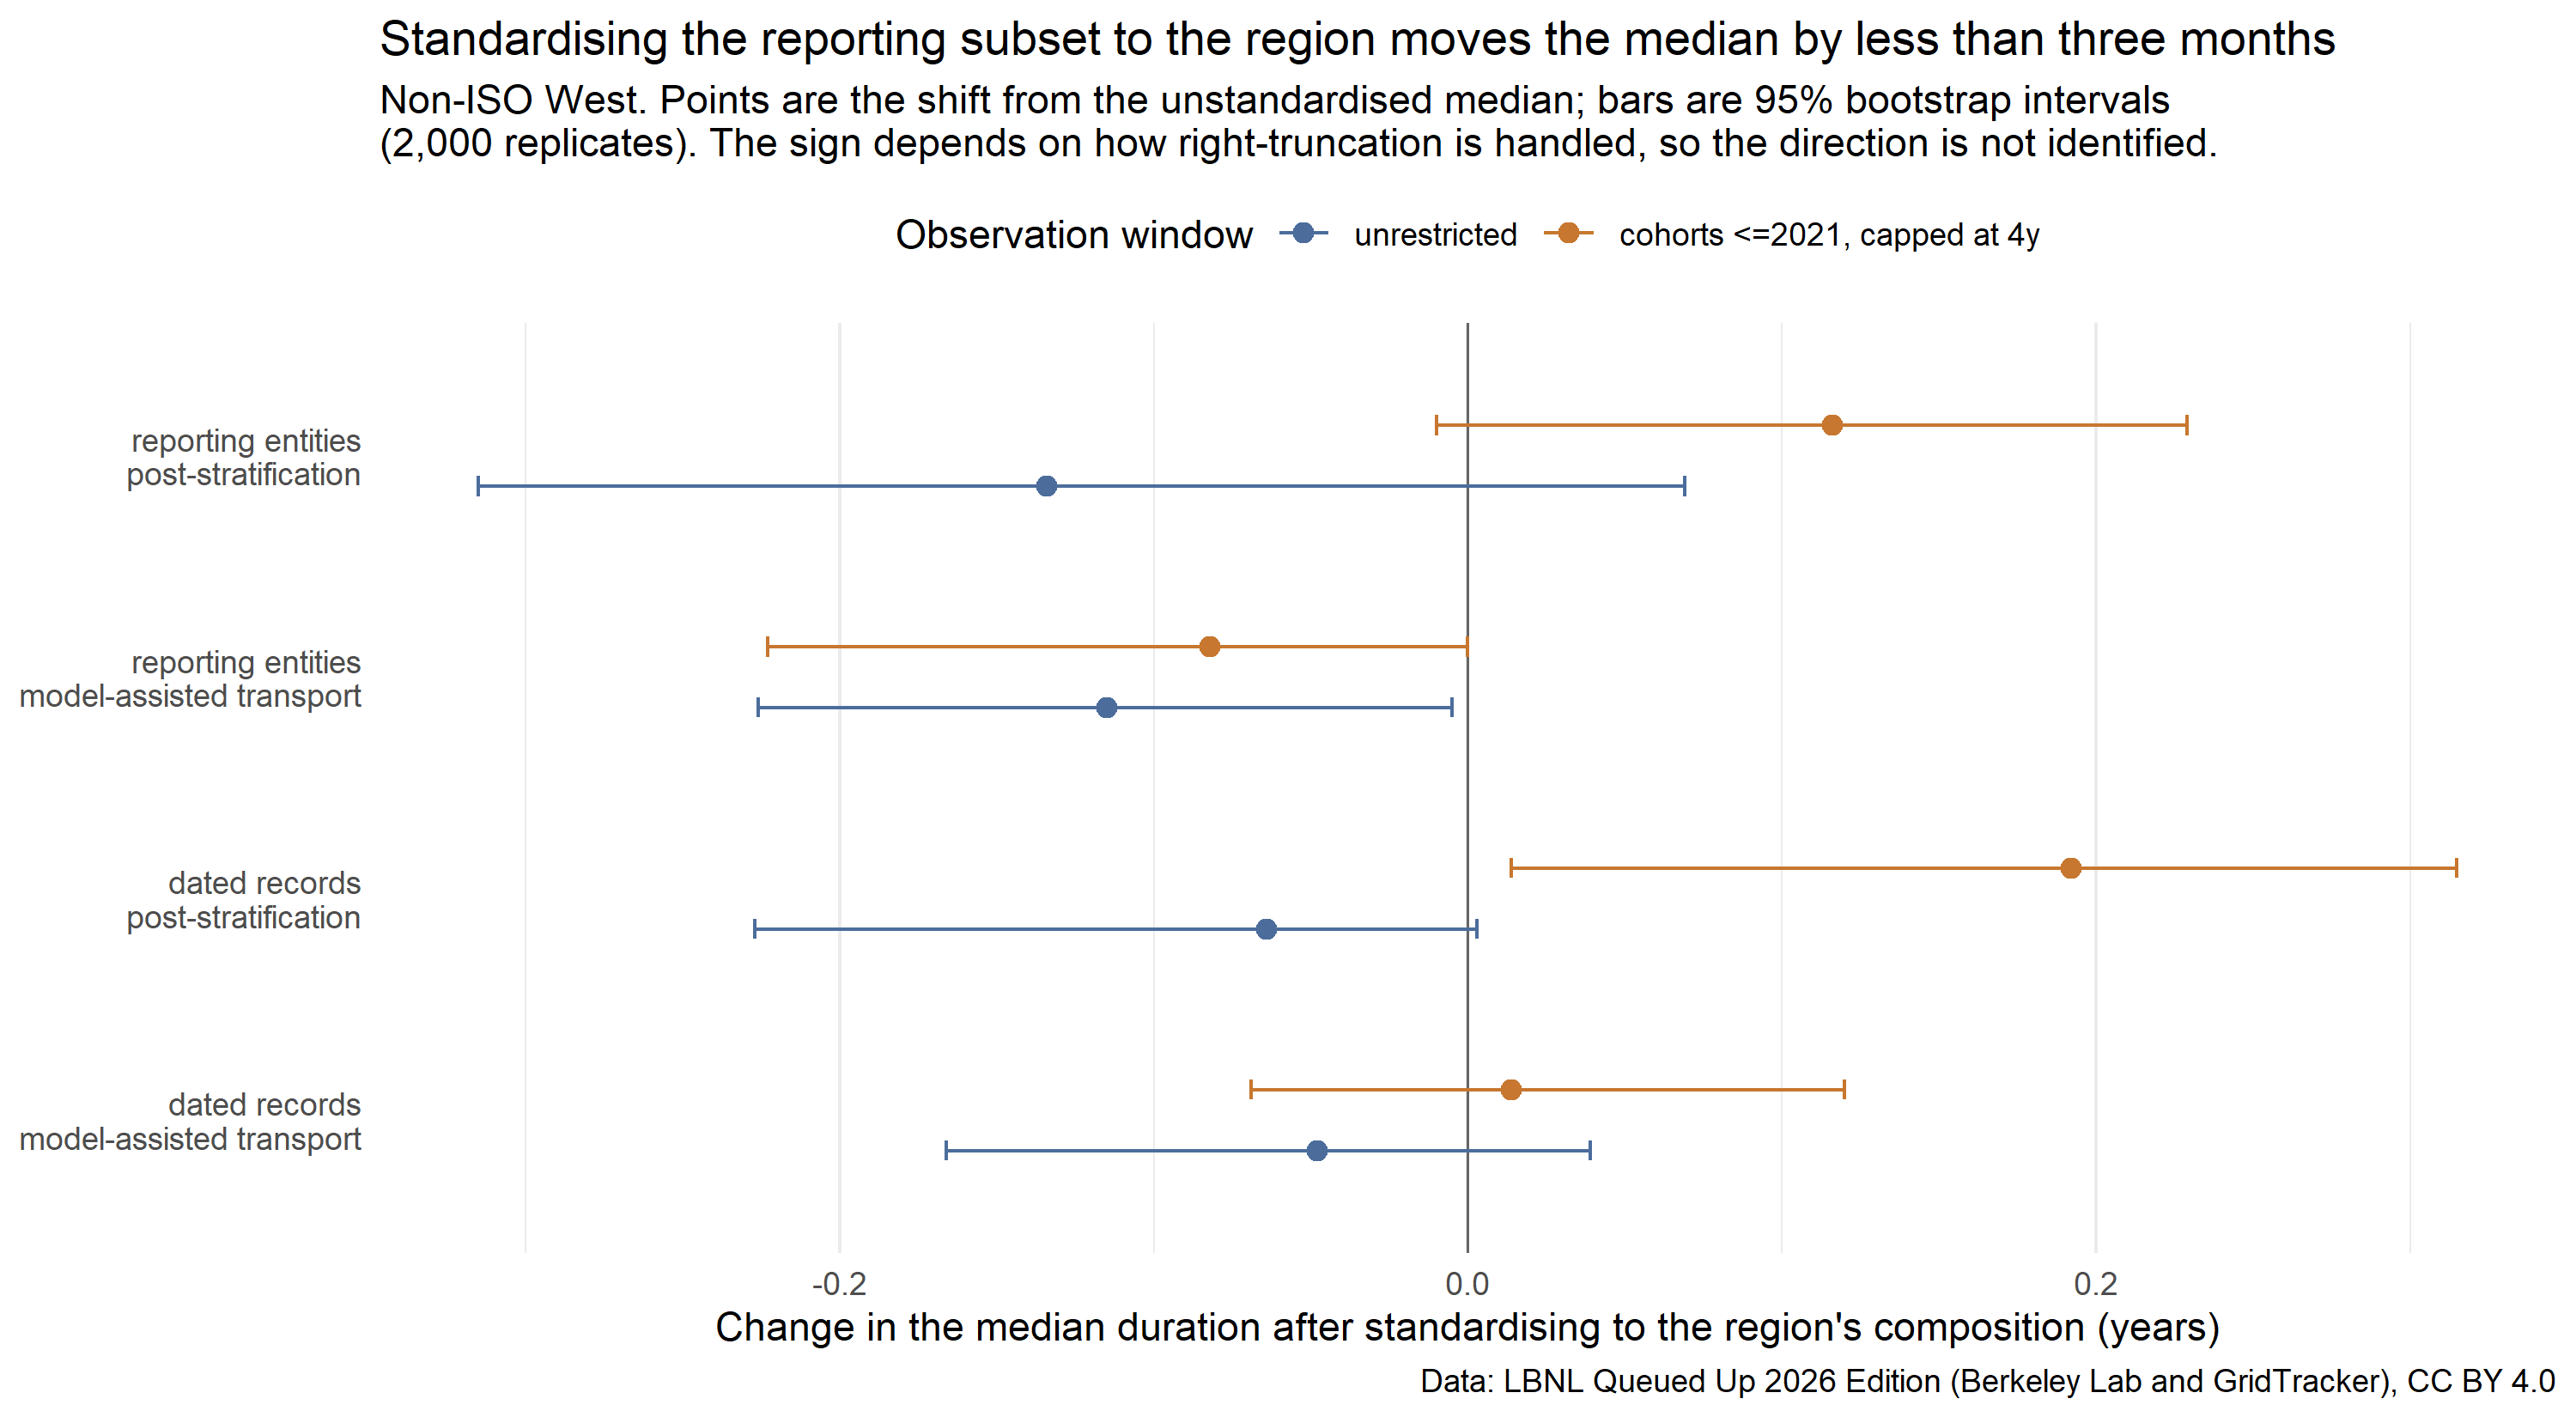
\includegraphics[width=\textwidth]{figures/05-bias-estimate.png}
\caption{Change in the median duration after standardising to the region's
composition, with \SI{95}{\percent} bootstrap intervals.}
\end{figure}

\subsection{Why the sign is not identified}

Duration here is not a complete measurement. A request entering the queue in 2023
cannot display a five-year withdrawal duration, because five years have not
elapsed. The observation window is bounded above by the file's cutoff, and that
bound bites harder on recent cohorts.

This interacts directly with the composition gap. The 2022+ cohort is
\SI{25.7}{\percent} of the regional population but only \SI{14.3}{\percent} of
the dated subset. Reweighting therefore transfers a quarter of the weight onto
the cohort whose durations are most severely truncated---which mechanically pulls
the median down, regardless of any genuine difference in how long those projects
take.

The matched window removes that mechanism: restricting to cohorts entering by
2021 gives every remaining record at least four years of exposure, and capping
durations at four years makes the measurement identical across cohorts. Under
that restriction the shift is positive.

Both estimates are defensible and they disagree. The unrestricted estimate
targets exactly the quantity \emph{Queued Up} publishes, and inherits its
truncation. The matched estimate is a cleaner contrast but describes a different,
more restricted quantity, discarding \SI{26}{\percent} of the regional population
to get there. Neither is wrong; they answer slightly different questions, and the
answers have opposite signs.

The honest reading is therefore: \textbf{the compositional bias in the published
western median is small---under three months on any specification, and under one
month on the specification that matches the published estimand---and its
direction is not identified by this data.} Given the validation result in Table~5,
which puts the compositional bias at about eight days when measured against a
known truth, the small magnitude is the robust finding and the sign is noise
around it.

\section{Withdrawal as a binary outcome}

The duration analysis is confined to \SI{12}{\percent} of western withdrawals.
Withdrawal \emph{itself} is recorded for every request, so a model of whether a
request is withdrawn can use the entire region without needing a single date.
This is a different question---what predicts withdrawal, not how long it
takes---but it is answerable on the full population, and it speaks to how much of
the variation in queue outcomes is attributable to the provider.

\subsection{Specification}

The outcome is withdrawal against everything else (active, operational,
suspended, unknown). Predictors are technology (six groups, solar as reference),
log capacity, cohort (four bins) and entity. Of \num{8097} requests, \num{7991}
have complete predictors; the 106 exclusions all lack a queue year.

Entity requires care. Seven providers, covering 90 requests, show no variation in
the outcome---five have no withdrawals at all, two have nothing but---and so
cannot be assigned an identified coefficient in a fixed-effects logistic model.
The primary specification therefore treats entity as a random intercept, which
shrinks such providers toward the grand mean rather than dropping them, and
retains all \num{7991} requests. A fixed-effects fit, with those seven providers
dropped and providers under 25 requests pooled, is reported alongside; so are
fits dropping the ambiguous suspended and unknown statuses, and restricting to
cohorts with at least four years of exposure.

\subsection{Results}

\begin{table}[htbp]
\centering
\caption{Odds of withdrawal, mixed-effects logistic ($n = \num{7991}$). Entity
variance 1.159 (SD 1.077); intraclass correlation \textbf{0.261}.}
\begin{tabular}{lrlr}
\toprule
Term & Odds ratio & \SI{95}{\percent} CI & $p$ \\
\midrule
Wind (vs Solar)   & 0.547 & $[0.458, 0.652]$ & $1.9\times10^{-11}$ \\
Solar+Battery     & 0.578 & $[0.487, 0.685]$ & $2.7\times10^{-10}$ \\
Battery           & 0.521 & $[0.428, 0.635]$ & $9.9\times10^{-11}$ \\
Gas               & 0.355 & $[0.282, 0.447]$ & $9.5\times10^{-19}$ \\
Other             & 0.314 & $[0.264, 0.373]$ & $4.6\times10^{-39}$ \\
log capacity (MW) & 1.129 & $[1.089, 1.170]$ & $3.2\times10^{-11}$ \\
cohort 2015--18 (vs $\leq$2014) & 0.610 & $[0.516, 0.721]$ & $7.6\times10^{-9}$ \\
cohort 2019--21   & 0.446 & $[0.374, 0.531]$ & $2.0\times10^{-19}$ \\
cohort 2022+      & 0.344 & $[0.293, 0.403]$ & $1.7\times10^{-39}$ \\
\bottomrule
\end{tabular}
\end{table}

Three findings.

\textbf{Solar is the most withdrawal-prone technology in the western queue.}
Every other group carries lower odds of withdrawal, from wind and storage at
roughly half solar's odds to gas and the miscellaneous group at about a third.
The coefficients are stable to every alternative specification: the fixed-effects
fit reproduces them to within 0.01, and dropping suspended and unknown statuses
changes nothing material.

\textbf{Larger projects are more likely to be withdrawn}, at 1.13 times the odds
per unit of log capacity---roughly \SI{9}{\percent} higher odds per doubling of
nameplate capacity. This strengthens to 1.18 under the equal-exposure
restriction.

\textbf{About a quarter of the latent variation in withdrawal risk sits between
providers.} The intraclass correlation of 0.261 says that a project's odds of
withdrawal depend substantially on whose queue it is in, after accounting for
what kind of project it is, how big it is and when it entered. The provider
random effect has a standard deviation of 1.077 on the log-odds scale, comparable
to the largest technology contrast in the table---the miscellaneous group, at
1.158---and larger than every other.

That last result matters for the paper's main question. It establishes that
providers differ materially in queue outcomes even conditional on observable
project attributes. It does not establish that they differ in withdrawal
\emph{timing}---the two are distinct, and timing is what the published median
measures. But it removes any comfortable presumption that providers are
interchangeable once technology and cohort are controlled for, which is exactly
the presumption the compositional correction in Section~\ref{sec:standardise} has
to make.

\subsection{The cohort coefficients are exposure, not behaviour}

The declining odds across cohorts should not be read as a falling propensity to
withdraw. They are dominated by exposure time.

\begin{table}[htbp]
\centering
\caption{Withdrawal rate and exposure time by cohort.}
\begin{tabular}{lrrrr}
\toprule
Cohort & Requests & Withdrawn & Rate & Median years of exposure \\
\midrule
$\leq$2014 & \num{2752} & \num{2084} & \SI{75.7}{\percent} & 17 \\
2015--18   & \num{1457} & \num{1060} & \SI{72.8}{\percent} & 9 \\
2019--21   & \num{1263} & \num{770}  & \SI{61.0}{\percent} & 6 \\
2022+      & \num{2519} & \num{1353} & \SI{53.7}{\percent} & 3 \\
\bottomrule
\end{tabular}
\end{table}

A request filed in 2024 has had two years in which to be withdrawn; one filed in
2010 has had fifteen. Restricting to cohorts with at least four years of exposure
attenuates the cohort coefficients (2019--21 moves from 0.446 to 0.539) without
touching the technology or capacity results, which is what one would expect if
the cohort gradient is largely an artefact of the observation window and the
others are not. The substantive findings survive; the cohort gradient should be
read as censoring.

\subsection{What carries the prediction}

\begin{table}[htbp]
\centering
\caption{Model comparison.}
\begin{tabular}{lr}
\toprule
Model & AIC \\
\midrule
project attributes only & \num{9752.1} \\
entity only             & \num{9816.8} \\
both                    & \num{9378.6} \\
\bottomrule
\end{tabular}
\end{table}

Neither project attributes nor provider identity subsumes the other; both
contribute (likelihood-ratio $\chi^2 = 456.2$ on 9 df for adding attributes to an
entity-only model). In-sample accuracy at a 0.5 threshold is \SI{71.1}{\percent}
against a \SI{65.9}{\percent} base rate---a modest improvement, consistent with
the general picture that recorded attributes explain a limited share of queue
outcomes.

\section{Limitations}

\textbf{The provider process channel is unmeasured and unmeasurable here.} This
is the binding limitation. Section~\ref{sec:standardise} corrects for differences
in \emph{what kind of projects} the reporting providers handle. It cannot correct
for differences in \emph{how} they handle them. If PacifiCorp's withdrawal
process is systematically slower or faster than PSCo's for reasons not encoded in
technology, capacity, cohort or service type, that difference is invisible in
this file, because PacifiCorp's withdrawal dates do not exist. The finding that
\SI{26}{\percent} of latent withdrawal-risk variation is between providers makes
this channel a live concern rather than a formality, and it is entirely plausible
that it is larger than the compositional channel measured here. Establishing that
would require withdrawal dates from at least one large non-reporting
provider, and those are not in this data file. The realistic routes are archived
snapshots of the provider's own public queue postings, where a request that
disappears between two successive snapshots has its withdrawal date bounded to
the interval between them, or a direct request to the provider.

\textbf{The calibration assumes transportability.} Stage A estimates how
technology and cohort shift duration in CAISO, ISO-NE, MISO and PJM, and the
validation is conducted within those same regions. Applying those effects to the
West assumes the relationships carry over. Western interconnection processes
differ from ISO tariff processes in ways that could plausibly alter them. This
assumption is load-bearing only for the model-assisted transport estimator, which
the validation already disqualifies; the preferred post-stratification estimator
uses the ISO regions solely to establish that technology and cohort matter enough
to be worth stratifying on, and takes its cell values from western data.

\textbf{Right-truncation is bounded, not eliminated.} The matched window
addresses it, but capping at four years and discarding post-2021 cohorts is a
blunt instrument. A survival-analytic treatment---modelling time to withdrawal
with censoring for requests still active---would use the data more efficiently.
It was not attempted here because the censoring pattern is itself entangled with
the reporting problem: for non-reporting providers we know a request was
withdrawn but not when, which is neither a standard observation nor a standard
censoring event.

\textbf{Thin cells.} Eight of 24 standardisation cells hold fewer than five dated
records, carrying \SI{5.3}{\percent} of the target weight; two hold none,
carrying \SI{0.08}{\percent}. The bootstrap intervals reflect this, but a median
computed from three observations is a fragile input regardless of how its
uncertainty is propagated.

\textbf{Technology and cohort groupings are choices.} Six technology groups and
four cohort bins were fixed before estimation on the criteria stated in
Section~2---each cohort carrying at least \SI{14}{\percent} of target weight,
2019--21 isolated as the surge, 2022+ isolated as the truncation-dominated
bin---but finer or coarser schemes would give somewhat different numbers. Given
the validation result, no plausible alternative stratification would change the
magnitude conclusion.

\textbf{The outcome coding is a judgement.} Suspended (244 requests) and unknown
(10) are treated as not withdrawn. Dropping them entirely leaves the coefficients
essentially unchanged, so the choice is not consequential, but it is a choice.

\textbf{One data source, one vintage.} Everything rests on the 2026 Edition file.
Reporting practice changes; several providers that record nothing today may begin
to, and the composition of the reporting subset would change with them.

\section{Conclusion}

The published median withdrawal duration for the non-ISO West rests on
\SI{12.1}{\percent} of the region's withdrawals, filed with five or six of its
thirty-one transmission providers, in service territories covering a minority of
the region's queue. The largest western provider, PacifiCorp, contributes
\SI{31}{\percent} of the region's withdrawals and \SI{15}{\percent} of its
recorded withdrawal dates, having recorded a date for only \SI{6}{\percent} of
its own withdrawals.

That reporting subset is measurably unlike the region it represents. Its
technology mix, queue cohort distribution and interconnection service type all
differ at $p < 10^{-10}$; only project capacity does not.

Yet standardising the subset to the region's actual composition moves the median
by less than three months on any specification, and by about three weeks on the
one that matches the published estimand---with an interval that includes zero and
a sign that reverses under a truncation-matched window. A validation exercise
inside the well-covered ISO regions explains why: imposing the West's
compositional distortion on a population whose durations are fully observed
shifts the median by roughly eight days. Technology, cohort and capacity account
for under \SI{5}{\percent} of the variance in withdrawal duration, so a
composition gap, even a large and highly significant one, has little room to move
a median.

The practical conclusion is not that the published figure is wrong. It is that
the caveat usually attached to such figures---that the reporting subset might
have an unrepresentative project mix---is the wrong caveat, or at least the minor
one. The composition problem is real, statistically unambiguous, and small in
effect. The problem that remains is coverage itself: a statistic drawn from one
eighth of the population, concentrated in five providers, whose principal risk is
that those five may run their queues on a different clock from the twenty-six
that publish nothing. That risk cannot be quantified from this data file, and the
finding that a quarter of the latent variation in withdrawal risk sits between
providers suggests it should not be assumed away.

The most useful thing that could be done with this result is not a better
correction. It is a withdrawal date from BPA, Idaho Power, APS, NorthWestern, NV
Energy, WAPA or PacifiCorp.

\section*{Reproducing}

Requires R (tested on 4.6.1) with \texttt{readxl}, \texttt{dplyr},
\texttt{tidyr}, \texttt{ggplot2} and \texttt{lme4}. Open
\texttt{queue-analysis.Rproj} and run in order: \texttt{00-setup.R} (shared
definitions), \texttt{01-explore.R} (the original exploratory session, kept as a
record), \texttt{02-figures.R}, \texttt{03-differences.R},
\texttt{04-standardise.R}, \texttt{05-logistic.R}, \texttt{06-figures.R}.

\texttt{04-standardise.R} runs \num{2000} bootstrap replicates for each of eight
estimates and takes several minutes. Both it and \texttt{05-logistic.R} set a
seed (\texttt{20260906}), so results are exactly reproducible.

\section*{Data and licence}

\texttt{data/LBNL\_Ix\_Queue\_Data\_File\_thru2025.xlsx}, \emph{Queued Up} 2026
Edition, from \url{https://emp.lbl.gov/queues}. Licensed CC BY 4.0; attribution
to Lawrence Berkeley National Laboratory and GridTracker. The analysis code in
this repository is offered under the same terms.

This paper describes the data file as published and takes no position on the
methodology of \emph{Queued Up} itself, whose authors report what transmission
providers disclose and are explicit that coverage varies by region.

\end{document}
